\documentclass[12pt,a4paper]{article}
\usepackage[utf8]{inputenc}
\usepackage{amsmath}
\usepackage{amsfonts}
\usepackage{amssymb}
\usepackage{graphicx}
\usepackage[left=2.5cm,right=2.5cm,top=2.5cm,bottom=2.5cm]{geometry}
\title{\bf 2nd exercise of mechanical vibration}
\usepackage{indentfirst}
\setlength{\parindent}{2em}
\usepackage{listings}
\lstset{language=Matlab}
\begin{document}
\maketitle
There is a single degree of freedom damped spring oscillator system. Draw the curves of amplitude amplification factor $\beta$ and phase $\phi$ according to frequency ratio variation respectively, where$\lambda  \in [0,3],\zeta  = 0.1,0.2,0.7,1.0$  

\section{Analytic Method}
The expression for amplitude amplification factor $\beta$ is
\begin{equation}
\beta = \frac{1}{\sqrt{(1 - \lambda^2)^2+(2\zeta \lambda)^2}}
\end{equation}

The expression for phase $\phi$ is
\begin{equation}
tan \phi = \frac{2\zeta\lambda}{1-\lambda^2},\quad  \phi \in [0,\pi]
\end{equation}


\begin{figure}[h!]
\centering
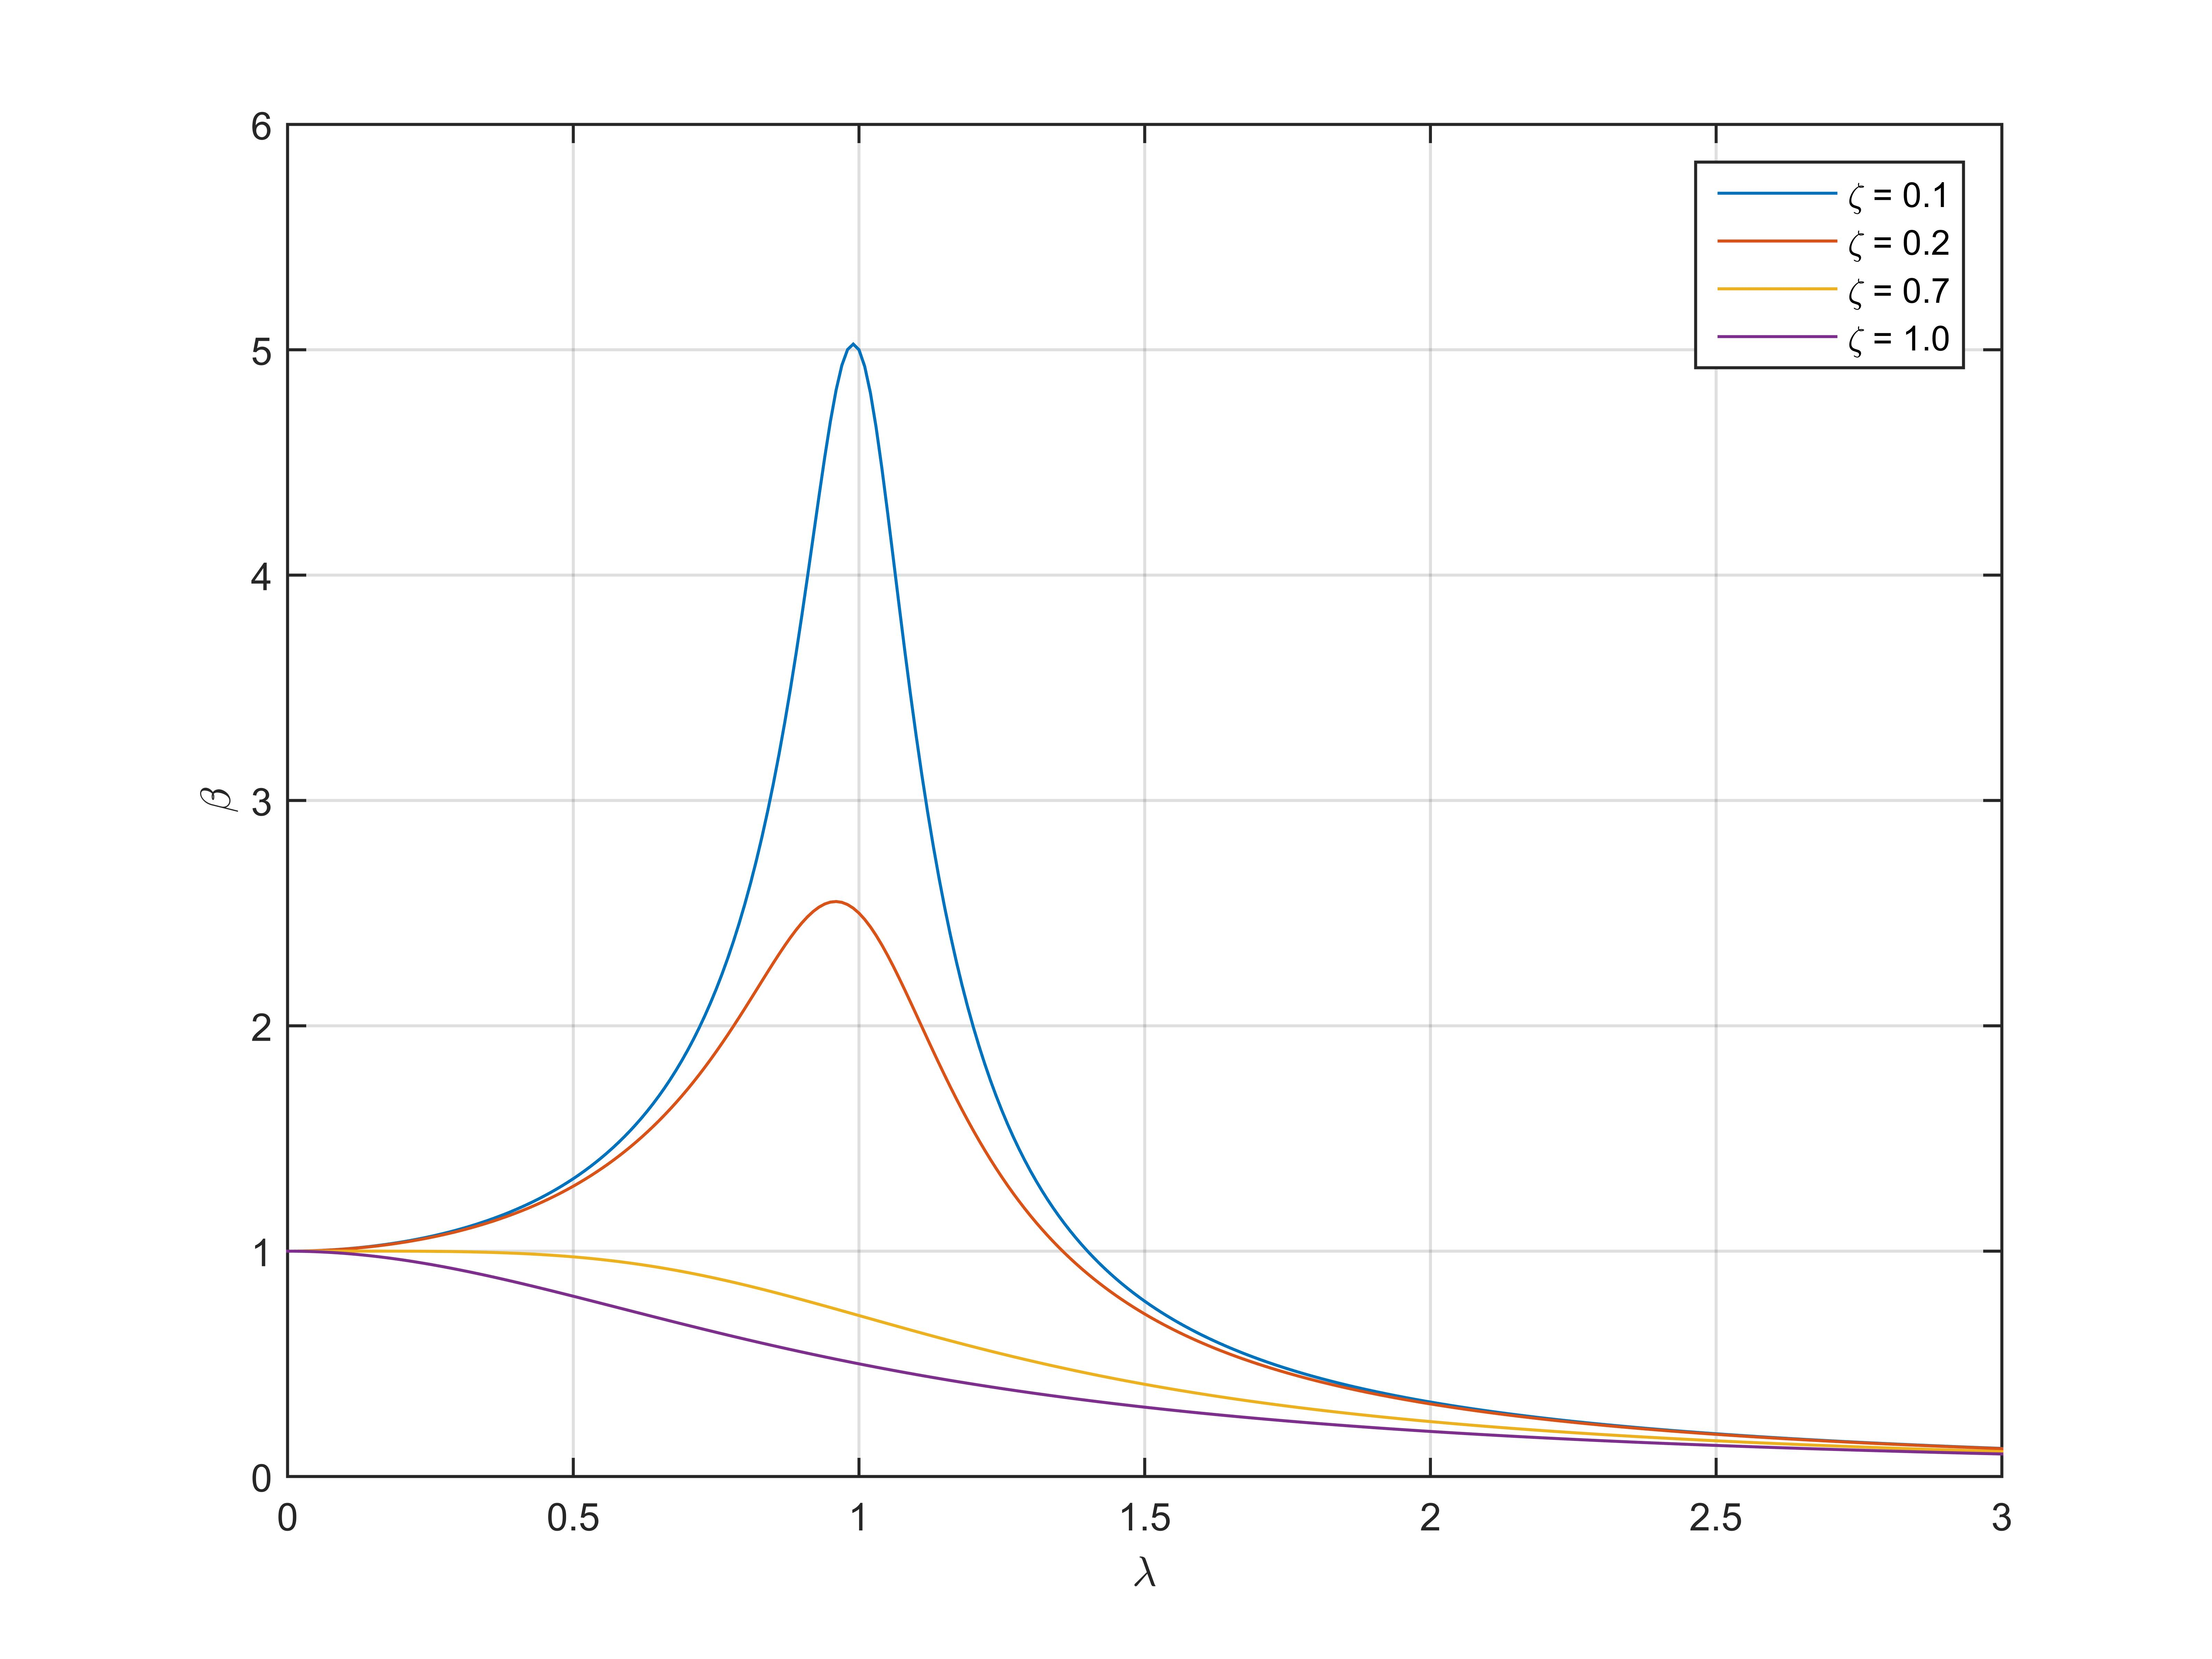
\includegraphics[width=0.7\linewidth]{source/bata_image}
\caption{$\beta{-}\zeta$ curve for $\lambda \in [0,3],\zeta = 0.1,0.2,0.7,1.0$}
\end{figure}

\begin{figure}[!h]
\centering
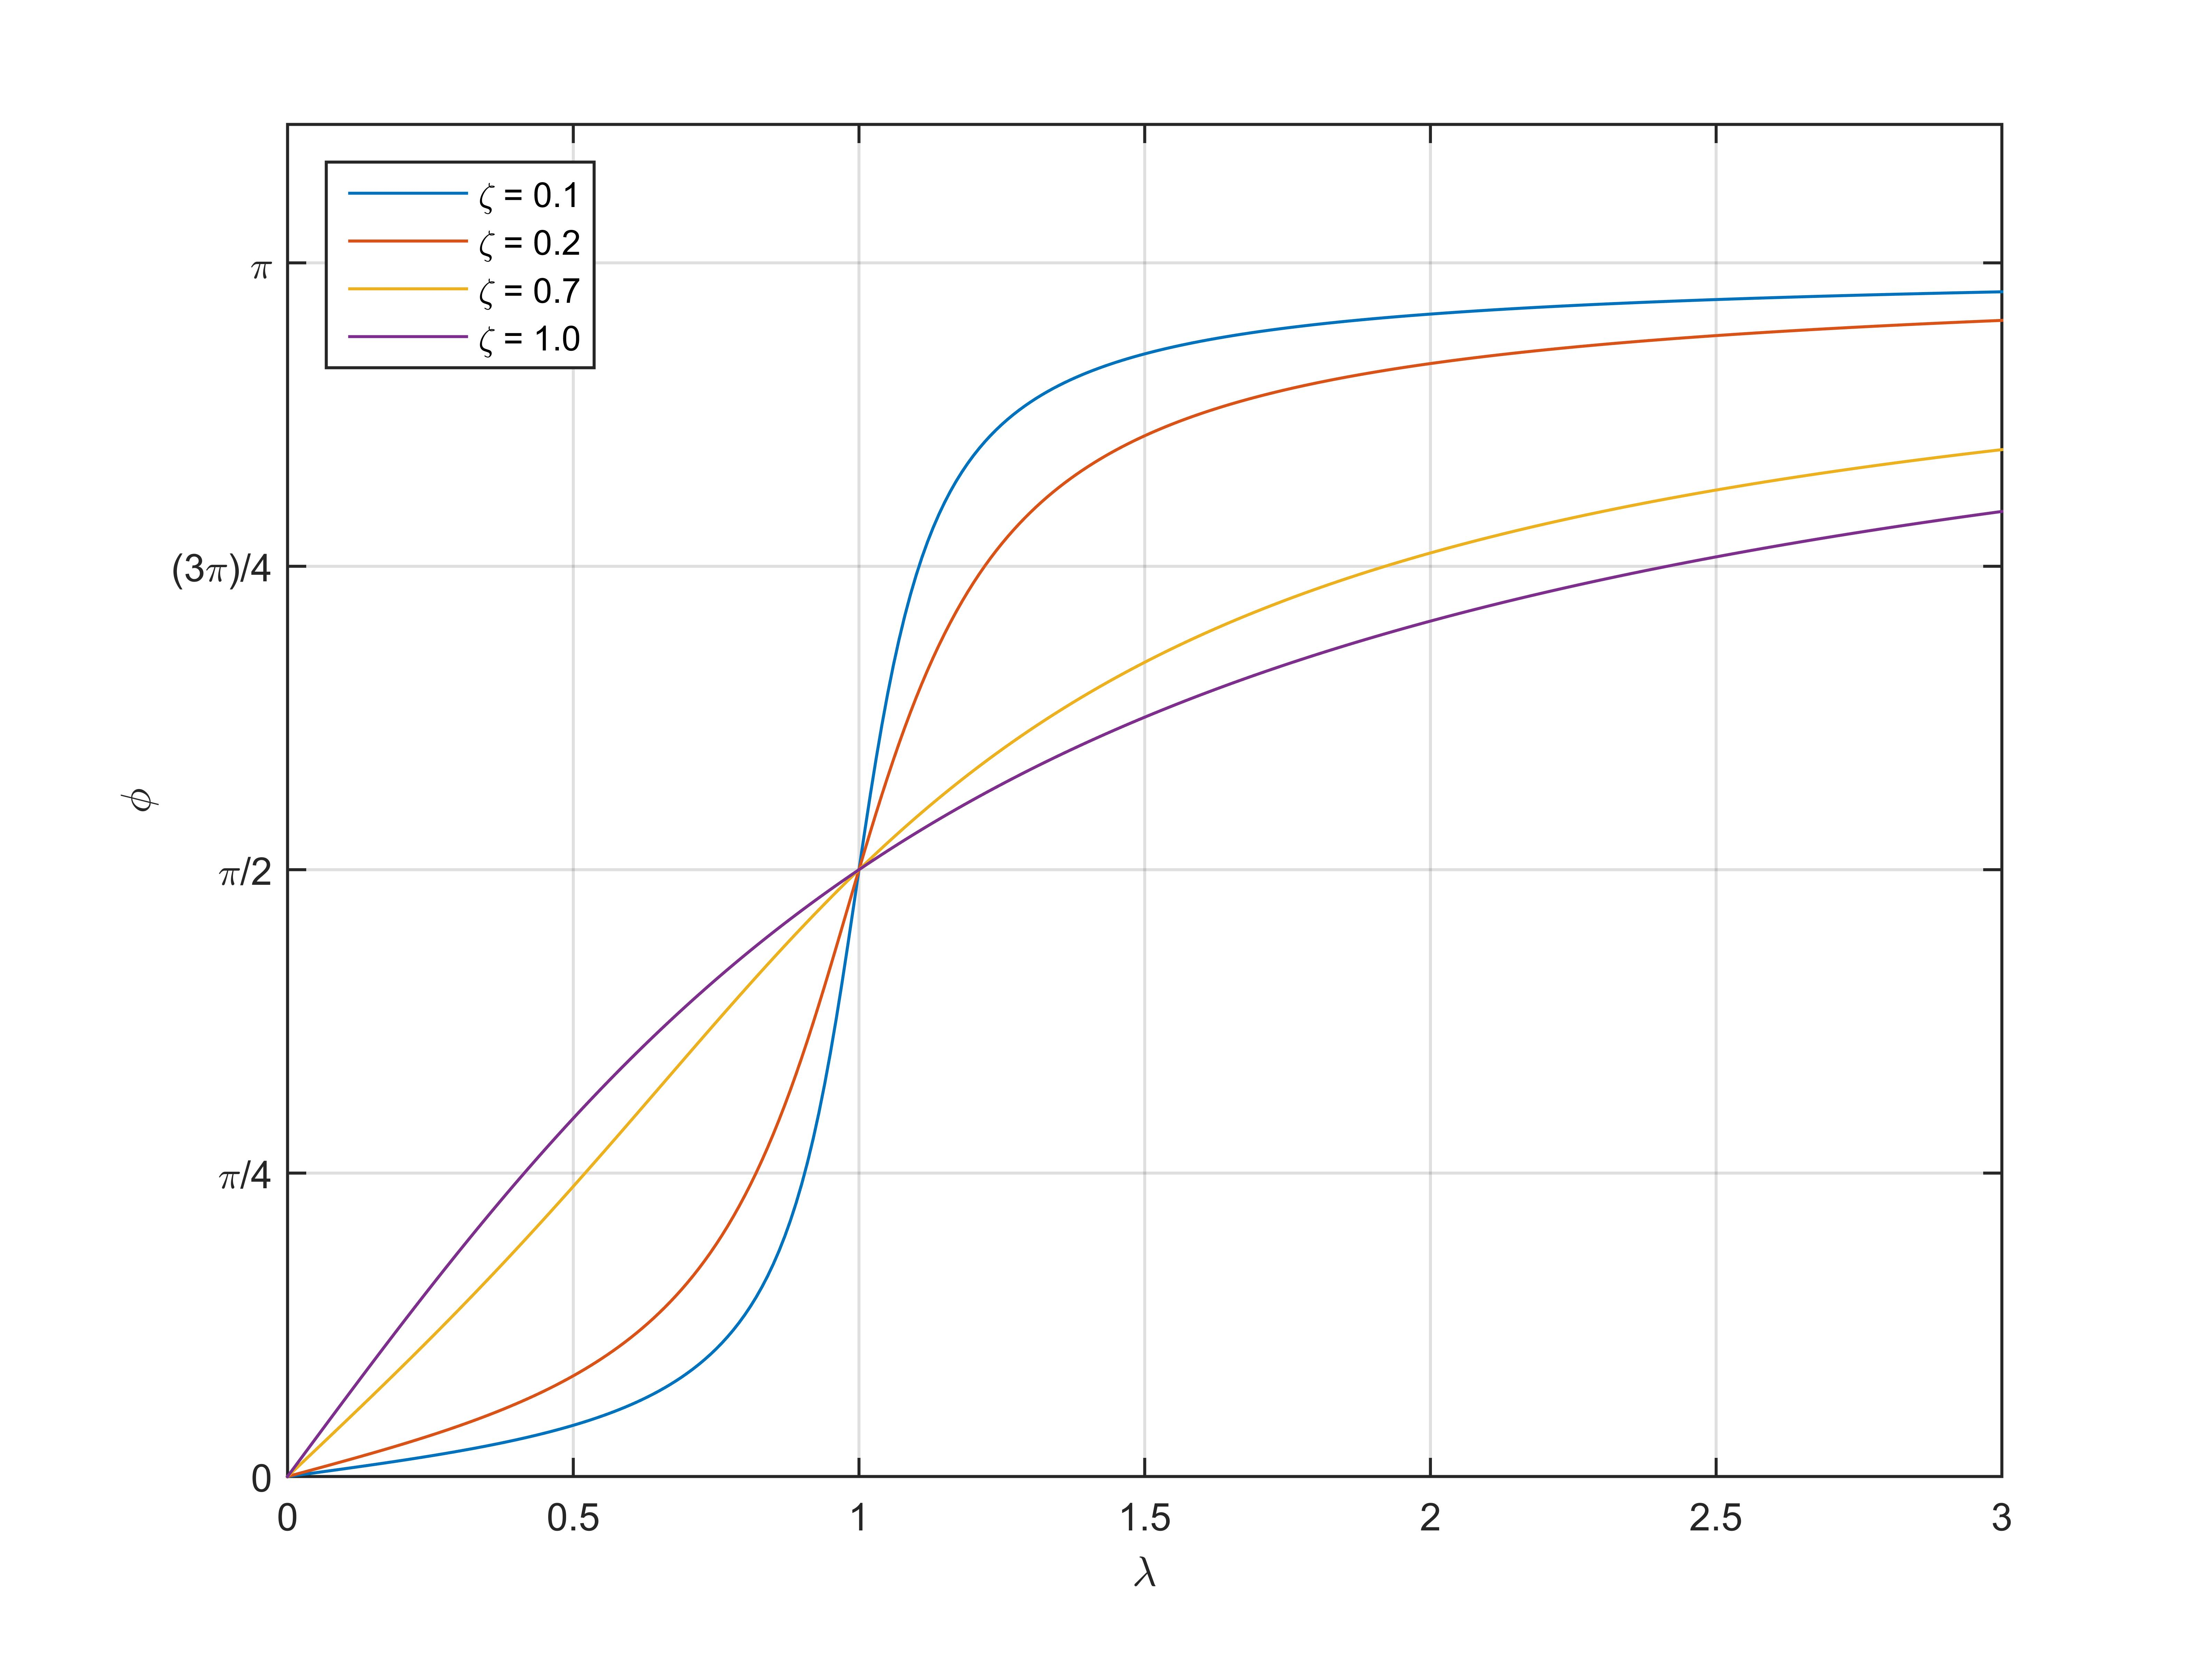
\includegraphics[width=0.7\linewidth]{source/phi_image}
\caption{$\phi{-}\zeta$ curve for $\lambda  \in [0,3],\zeta  = 0.1,0.2,0.7,1.0$}
\end{figure}
\section{Appendix}
\subsection{Analytic Method}
\begin{lstlisting}
clear all
lambda = 0:0.01:3;
zeta = [0.1,0.2,0.7,1.0];
for i = 1:size(zeta,2)
	beta(i,:) = 1./sqrt((1 - lambda.^2).^2+(2*zeta(i)*lambda).^2);
	phi(i,:) = atan((2*zeta(i)*lambda)./(1-lambda.^2));
    phi(i,find(phi(i,:)<0))=phi(i,find(phi(i,:)<0))+pi;
end
figure(1)
plot(lambda,beta);grid on;
xlabel('\lambda');
ylabel('\beta')
legend('\zeta = 0.1','\zeta = 0.2','\zeta = 0.7','\zeta = 1.0')
print -f -r800 -djpeg bata_image

figure(2)
plot(lambda,phi);grid on;
xlabel('\lambda');
ylabel('\phi')
legend('\zeta = 0.1','\zeta = 0.2','\zeta = 0.7','\zeta = 1.0','Location','northwest')
set(gca,'YTick',0:pi/4:pi)
set(gca,'YTickLabel',{'0','\pi/4','\pi/2','(3\pi)/4','\pi'})
print -f -r800 -djpeg phi_image
\end{lstlisting}
\end{document}